\section{Ý tưởng}
Mô hình không gian vector là một tiếp cận kinh điển nhưng vẫn đầy sức mạnh trong lĩnh vực truy xuất thông tin, nổi bật bởi khả năng ánh xạ ngôn ngữ tự nhiên vào không gian hình học trừu tượng, nơi mỗi thực thể ngôn ngữ -- bất kể là tài liệu hay truy vấn -- đều được biểu diễn như một \textbf{vector trọng số} trong một không gian nhiều chiều.

Trong không gian này, mỗi chiều tương ứng với một \textit{term} từ tập từ vựng đã được xây dựng trước đó. Nhờ đó, toàn bộ tập hợp tài liệu và truy vấn có thể được số hóa và đồng nhất hóa về mặt biểu diễn, tạo điều kiện thuận lợi cho việc so sánh, đối chiếu và xếp hạng. Cụ thể, ta có thể mô tả biểu diễn của một tài liệu \(d\) và truy vấn \(q\) thông qua các vector trọng số:

\begin{equation}
    \text{Rep}(d) = (w_{d1}, w_{d2}, \dots, w_{dN}), \quad \text{Rep}(q) = (w_{q1}, w_{q2}, \dots, w_{qN})
\end{equation}

trong đó mỗi trọng số \(w_{ij}\) phản ánh \textbf{mức độ quan trọng} của từ khóa thứ \(j\) trong văn bản hoặc câu truy vấn tương ứng. Trọng số này thường được tính theo các công thức như TF, TF-IDF hoặc các biến thể hiện đại hơn nhằm phản ánh độ đặc trưng và tính phân biệt của từ khóa.

Tại thời điểm truy vấn, hệ thống sẽ tính toán \textbf{độ tương đồng} giữa truy vấn và từng tài liệu trong tập hợp, sử dụng các độ đo hình học như \textbf{khoảng cách Euclid} hoặc phổ biến hơn là \textbf{độ đo cosine} -- một phép đo góc giữa hai vector nhằm xác định mức độ định hướng tương đồng giữa chúng trong không gian từ vựng. Kết quả của phép tính này là một giá trị đại diện cho mức độ phù hợp giữa tài liệu và truy vấn, được sử dụng để \textbf{xếp hạng} tài liệu theo thứ tự giảm dần về độ liên quan.

\begin{equation}
    \text{similarity}(\text{Rep}(d), \text{Rep}(q)) \rightarrow \text{ranking}
\end{equation}

Minh họa dưới đây cho ta cái nhìn trực quan về cách mà truy vấn và tài liệu được biểu diễn trong không gian hình học. Trong ví dụ, ba thuật ngữ: \textit{color}, \textit{vehicle}, \textit{motion} tạo thành không gian ba chiều, và tập hợp các từ được ánh xạ thành các vector tương ứng trong không gian đó:

\begin{figure}[H]
    \caption{Minh họa mô hình không gian vector}
    \begin{center}
        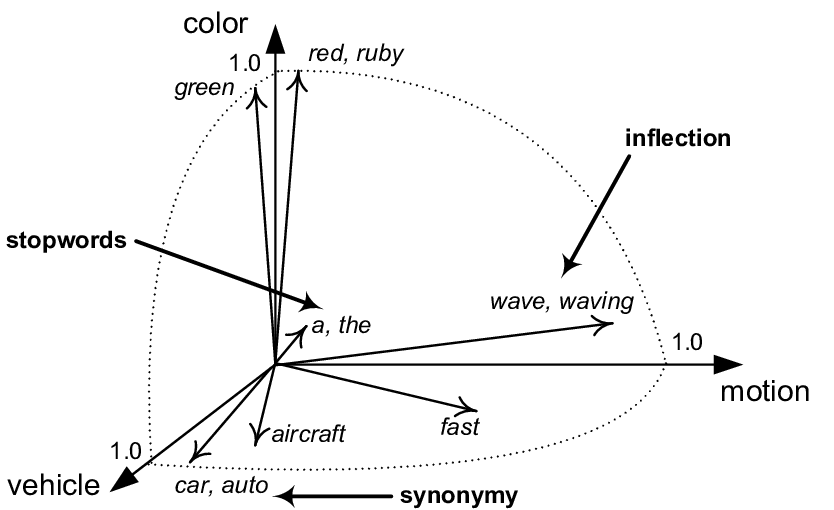
\includegraphics[width=\linewidth]{assets/vsm-illustration.png}
    \end{center}
\end{figure}

Mô hình không gian vector, với khả năng chuyển hóa văn bản thành hình khối đại số, đã khẳng định vai trò không thể thiếu trong nền tảng các hệ thống tìm kiếm hiện đại -- nơi sự phù hợp không chỉ nằm ở từ khóa chung, mà còn ở sự cộng hưởng định hướng giữa các biểu diễn toán học của ngôn ngữ.
